\documentclass[12pt,a4paper]{article}

\usepackage[utf8]{inputenc}
\usepackage[T1]{fontenc}
\usepackage{lmodern}
\usepackage{microtype}
\usepackage{geometry}
\usepackage{array}
\usepackage{booktabs}
\usepackage{longtable}
\usepackage{tabularx}
\usepackage{multirow}
\usepackage{float}
\usepackage[section]{placeins}
\usepackage[table]{xcolor}
\usepackage{enumitem}
\usepackage{pdflscape}
\usepackage{tikz}
\usepackage{hyperref}
\usepackage{fancyhdr}

\usetikzlibrary{arrows.meta,positioning}

\geometry{top=2.2cm,bottom=2.2cm,left=2.3cm,right=2.3cm}
\setlength{\parindent}{0pt}
\setlength{\parskip}{0.55em}
\renewcommand{\arraystretch}{1.25}
\renewcommand{\tablename}{Tabela}
\newcolumntype{L}[1]{>{\raggedright\arraybackslash}p{#1}}

\definecolor{azul}{HTML}{1F4E78}
\definecolor{azulclaro}{HTML}{D9EAF7}
\definecolor{cinzaclaro}{HTML}{F2F2F2}

\hypersetup{
  colorlinks=true,
  linkcolor=azul,
  urlcolor=azul,
  pdftitle={Plano de Verificação - Mini GPU SIMD},
  pdfauthor={Vinícius Carvalho Pimpim}
}
\urlstyle{tt}

\pagestyle{fancy}
\fancyhf{}
\lhead{Projeto Fase 2 - CI Digital}
\rhead{Plano de Verificação}
\cfoot{\thepage}
\setlength{\headheight}{15pt}

\newcommand{\req}[1]{\texttt{\detokenize{[#1]}}}
\newcommand{\signal}[1]{\texttt{\detokenize{#1}}}
\newcommand{\headingrow}[1]{%
  \rowcolor{azulclaro}\multicolumn{5}{l}{\textbf{#1}}\\
}

\title{\textbf{Desenvolvimento do Plano de Verificação Versão 1.1}\\[0.3em]
       \large Mini GPU SIMD Simplificada}
\author{Vinícius Carvalho Pimpim\\Projeto Fase 2 - CI Digital}
\date{}

\begin{document}

\maketitle

\section{Especificação}

O IP a ser desenvolvido no projeto final da Fase 2 consiste em uma GPU simplificada
baseada na lógica SIMD (\textit{Single Instruction, Multiple Data}). Nessa técnica de
computação paralela, uma mesma operação é aplicada simultaneamente a diferentes
elementos de dados. O objetivo do projeto é desenvolver um módulo capaz de acelerar
cálculos vetoriais simples por meio de quatro unidades aritméticas operando em paralelo.

A versão inicial processa dois vetores de quatro posições, com elementos de 8 bits. Cada
posição da memória vetorial armazena uma palavra de 32 bits, composta pelas quatro
\textit{lanes}. O conjunto inicial de operações inclui adição, subtração, multiplicação
e divisão.

\section{Linguagem utilizada}

O projeto será desenvolvido em \textbf{SystemVerilog}. A linguagem será utilizada
tanto para a descrição dos módulos de hardware quanto para a implementação do
ambiente de verificação.

O ambiente de verificação UVM também será implementado em SystemVerilog.

\begin{table}[H]
  \centering
  \caption{Uso de SystemVerilog no projeto.}
  \begin{tabularx}{\textwidth}{l X}
    \toprule
    \textbf{Parte do projeto} & \textbf{Utilização} \\
    \midrule

    RTL &
    Descrição sintetizável dos módulos que formam a mini GPU. \\

    Testbench Inicial &
    Geração dos pacotes de 42 bits e dos demais estímulos de entrada. \\
    
    Assertions &
    Verificação dos handshakes, sinais de controle e transições da FSM. \\

    Cobertura &
    Verificação dos opcodes, tipos de pacote, endereços e casos de borda
    exercitados durante os testes. \\

    \bottomrule
  \end{tabularx}
\end{table}

O código executado pelo host não faz parte do escopo inicial da implementação.
Para a verificação, o comportamento do host será representado pelo testbench,
que enviará diretamente os pacotes de requisição de 42 bits.




\subsection{Parâmetros da arquitetura}

\begin{table}[ht]
  \centering
  \caption{Parâmetros principais da mini GPU.}
  \begin{tabularx}{\textwidth}{>{\bfseries}l X}
    \toprule
    Parâmetro & Valor \\
    \midrule
    Interface de requisição do host & Pacote de 42 bits com protocolo \\
    Interface de resposta ao host & Dados de 32 bits Resposta de um comando \\
    Barramento interno & AXI4-Lite, dados de 32 bits \\
    Número de \textit{lanes} & 4 \\
    Largura de cada elemento & 8 bits, sem sinal \\
    Palavra vetorial & 32 bits \\
    Memória vetorial & 256 palavras de 32 bits \\
    Endereço interno da memória & 8 bits \\
    Pacote interno de requisição & 42 bits: \signal{TYPE[1:0]} + \signal{PAYLOAD[39:0]} \\
    Número de comandos simultâneos & 1 \\
    \bottomrule
  \end{tabularx}
\end{table}

\FloatBarrier
\clearpage
\section{Arquitetura}

\begin{figure}[H]
\centering
\resizebox{0.92\textwidth}{!}{%
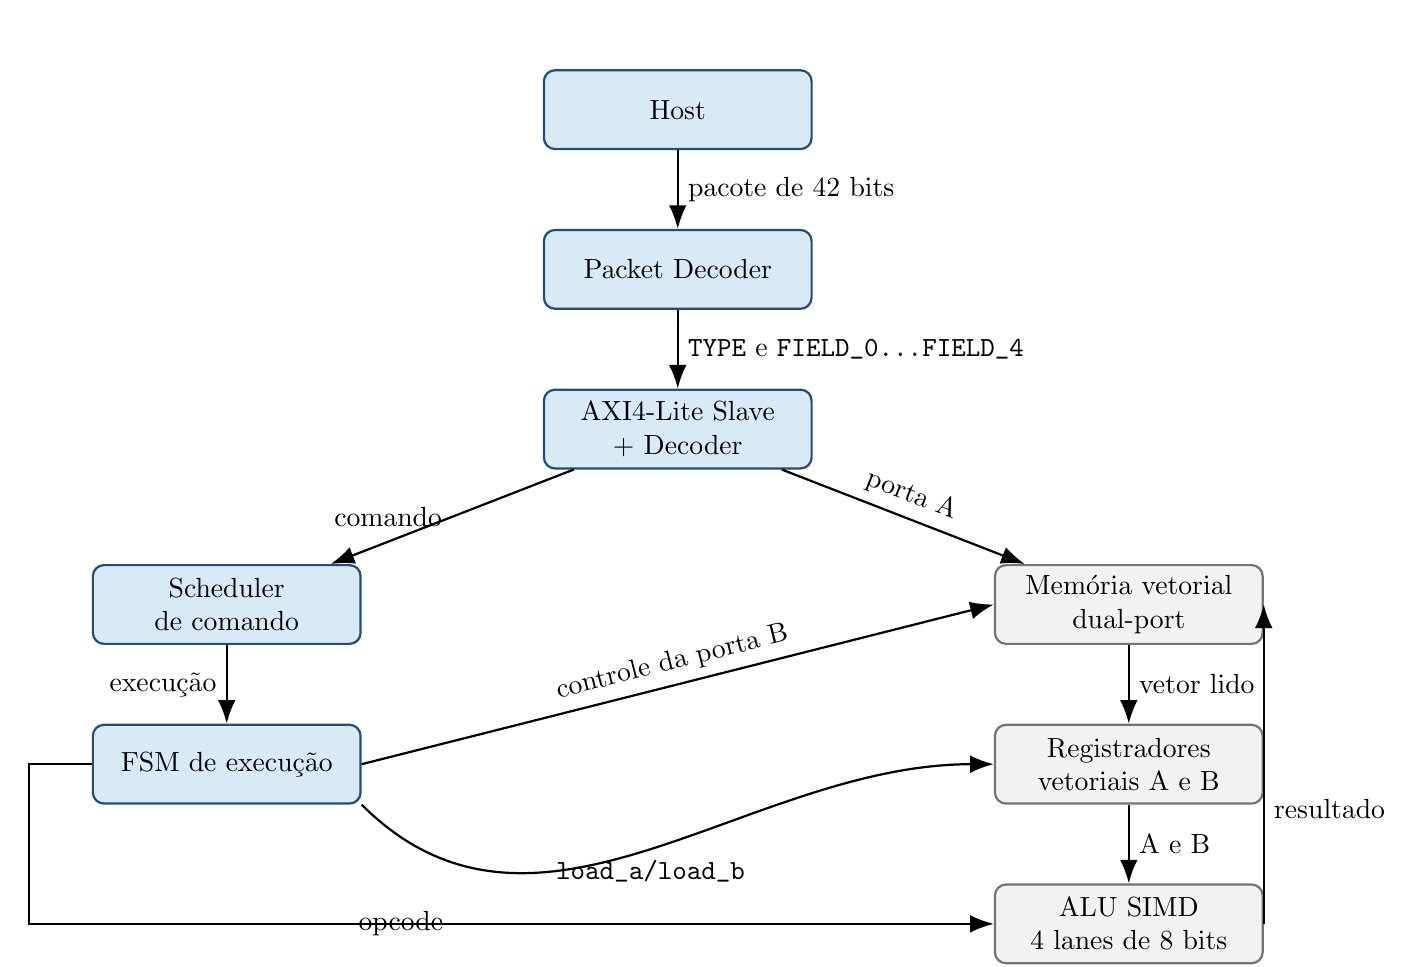
\begin{tikzpicture}[
  block/.style={draw=azul, thick, rounded corners, align=center,
                minimum width=3.4cm, minimum height=1.0cm, fill=azulclaro},
  data/.style={draw=black!55, thick, rounded corners, align=center,
               minimum width=3.4cm, minimum height=1.0cm, fill=cinzaclaro},
  arrow/.style={-{Latex[length=3mm]}, thick},
  node distance=1.0cm and 2.0cm
]
  \node[block] (host) {Host};
  \node[block, below=of host] (packet) {Packet Decoder};
  \node[block, below=of packet] (axis) {AXI4-Lite Slave\\+ Decoder};
  \node[block, below left=1.2cm and 2.3cm of axis] (scheduler) {Scheduler\\de comando};
  \node[block, below=of scheduler] (fsm) {FSM de execução};
  \node[data, below right=1.2cm and 2.3cm of axis] (mem) {Memória vetorial\\dual-port};
  \node[data, below=of mem] (regs) {Registradores\\vetoriais A e B};
  \node[data, below=of regs] (alu) {ALU SIMD\\4 lanes de 8 bits};

  \draw[arrow] (host) -- node[right]{pacote de 42 bits} (packet);
  \draw[arrow] (packet) -- node[right]{\signal{TYPE} e \signal{FIELD_0...FIELD_4}} (axis);
  \draw[arrow] (axis) -- node[left]{comando} (scheduler);
  \draw[arrow] (scheduler) -- node[left]{execução} (fsm);
  \draw[arrow] (axis) -- node[above, sloped]{porta A} (mem);
  \draw[arrow] (fsm.east) -- node[above, sloped]{controle da porta B} (mem.west);
  \draw[arrow] (mem) -- node[right]{vetor lido} (regs);
  \draw[arrow] (regs) -- node[right]{A e B} (alu);
  \draw[arrow] (fsm.south east) to[out=-45,in=180]
    node[midway,below]{\signal{load_a/load_b}} (regs.west);
  \draw[arrow] (fsm.west) -- ++(-0.8,0) |-
    node[pos=0.72,left]{opcode} (alu.west);
  \draw[arrow] (alu.east) -| node[pos=0.68,right]{resultado} (mem.east);
\end{tikzpicture}}
\caption{Arquitetura funcional da mini GPU SIMD.}
\end{figure}

\subsection{Descrição dos blocos}

\subsubsection{Packet Decoder}

É a porta de entrada das requisições do host. O bloco recebe o pacote de 42 bits. O Packet Decoder não acessa a memória nem o
Scheduler diretamente; sua única responsabilidade é entregar uma representação
decodificada e estável diretamente ao AXI4-Lite Slave Decoder.

\subsubsection{AXI4-Lite Slave Decoder}

Recebe diretamente do Packet Decoder o tipo e os cinco campos desempacotados.
O bloco interpreta a requisição, calcula o endereço interno correspondente e
seleciona \signal{CONTROL} e \signal{COMMAND} ou a
memória vetorial.

\subsubsection{Memória vetorial dual-port}

Memória com duas interfaces independentes de leitura e escrita. A porta A é
controlada pelo AXI4-Lite Slave Decoder, e a porta B é controlada pela FSM. Cada endereço
armazena um vetor completo de 32 bits.

\subsubsection{Scheduler de comando}

Recebe do AXI4-Lite Slave Decoder o opcode, os endereços dos vetores A e B e o endereço de
destino. O Scheduler armazena um comando, controla os sinais \signal{BUSY} e
\signal{DONE}, via registrador de STATUS e entrega o comando à FSM.
\signal{valid/ready}.

\subsubsection{FSM de execução}

Controla a leitura dos dois operandos, o carregamento dos registradores, a execução
da ALU e a escrita do resultado. A sequência de estados é apresentada na
Tabela~\ref{tab:fsm}.

\begin{table}[ht]
  \centering
  \caption{Estados da FSM de execução.}
  \label{tab:fsm}
  \begin{tabularx}{\textwidth}{>{\ttfamily}l X}
    \toprule
    \normalfont\textbf{Estado} & \textbf{Descrição} \\
    \midrule
    IDLE & Aguarda um comando válido do Scheduler. \\
    READ\_A & Coloca \signal{SRC_A} no endereço de leitura da memoria porta B e solicita leitura. \\
    LOAD\_A & Ativa \signal{load_a} e carrega no registrador o vetor devolvido pela memoria. \\
    READ\_B & Coloca \signal{SRC_B} no endereço de leitura da memoria porta B e solicita leitura. \\
    LOAD\_B & Ativa \signal{load_b} e carrega no registrador o vetor devolvido pela memoria. \\
    EXECUTE & Mantém os operandos e o opcode estáveis para a ALU SIMD. \\
    WRITE\_RESULT & Escreve o resultado da ALU no endereço \signal{DST}. \\
    FINISH & Gera \signal{exec_done} por um ciclo e retorna a \signal{IDLE}. \\
    \bottomrule
  \end{tabularx}
\end{table}

\subsubsection{Registradores vetoriais A e B}

Armazenam os dois vetores lidos da porta B da memória. O barramento de 32 bits
proveniente da memória alimenta os dois registradores, e a FSM seleciona o destino
por meio de \signal{load_a} e \signal{load_b}.

\subsubsection{ALU SIMD com quatro lanes de 8 bits}

Composta por quatro ALUs simples de 8 bits. As quatro unidades recebem o mesmo
opcode e operam simultaneamente sobre posições independentes dos vetores A e B.

\clearpage
\section{Interfaces dos blocos}

As tabelas apresentam somente os sinais necessários entre os blocos. Barramentos
de dados são conectados diretamente ao bloco que os utiliza; a FSM permanece
responsável apenas pelos sinais de controle.

\subsection{Packet Decoder}

\begin{table}[H]
  \centering
  \caption{Interface do Packet Decoder.}
  \small
  \begin{tabularx}{\textwidth}
    {L{0.29\textwidth} L{0.16\textwidth} L{0.10\textwidth} X}
    \toprule
    \textbf{Sinal} & \textbf{Tipo} & \textbf{Largura} & \textbf{Descrição} \\
    \midrule
    \signal{clk/rst}
      & Input
      & 1 cada
      & Clock e reset do bloco. \\

    \signal{req_payload}
      & Input
      & 42
      & Pacote de requisição enviado pelo host. \\

    \signal{req_valid/ready}
      & Input/Output
      & 1 cada
      & Handshake com o host. \\

    \signal{decoded_valid/ready}
      & Output/Input
      & 1 cada
      & Handshake com o AXI4-Lite Slave Decoder. \\

    \signal{req_type}
      & Output
      & 2
      & Cópia de \signal{req_payload[41:40]}. \\

    \signal{field_0} a \signal{field_4}
      & Output
      & $5\times8$
      & Cópias dos cinco campos de 8 bits do pacote. \\
    \bottomrule
  \end{tabularx}
\end{table}


\subsection{AXI4-Lite Slave Decoder}

\begin{table}[H]
  \centering
  \caption{Interface do AXI4-Lite Slave Decoder.}
  \small
  \begin{tabularx}{\textwidth}
    {L{0.29\textwidth} L{0.16\textwidth} L{0.10\textwidth} X}
    \toprule
    \textbf{Sinal} & \textbf{Tipo} & \textbf{Largura} & \textbf{Descrição} \\
    \midrule
    \signal{clk/rst}
      & Input
      & 1 cada
      & Clock e reset. \\

    \signal{decoded_valid/ready}
      & Input/Output
      & 1 cada
      & Handshake com o Packet Decoder. \\

    \signal{req_type + fields}
      & Input
      & 2 e $5\times8$
      & Tipo e cinco campos desempacotados. \\

    \signal{rsp_*}
      & Output
      & 32, 1 e 1
      & \signal{rsp_data}, \signal{rsp_valid} e \signal{rsp_error}. \\

    \signal{mem_a_addr/wdata}
      & Output
      & 8 e 32
      & Endereço e vetor enviados à porta A. \\

    \signal{mem_a_we/re}
      & Output
      & 1 cada
      & Habilitações da porta A. \\

    \signal{mem_a_rdata}
      & Input
      & 32
      & Vetor lido pela porta A. \\

    \signal{cmd_fields}
      & Output
      & 32
      & OPCODE, SRCA, SRCB, DST \\

    \signal{cmd_valid}
      & Output
      & 1
      & Pulso enviado ao Scheduler quando chega \signal{GPU_START}. \\

    \signal{cmd_ready/busy/done}
      & Input
      & 1 cada
      & Prontidão e estado fornecidos pelo Scheduler. \\
    \bottomrule
  \end{tabularx}
  
\end{table}


\subsection{Scheduler}

\begin{table}[H]
  \centering
  \caption{Interface do Scheduler.}
  \small
  \begin{tabularx}{\textwidth}
    {L{0.29\textwidth} L{0.16\textwidth} L{0.10\textwidth} X}
    \toprule
    \textbf{Sinal} & \textbf{Tipo} & \textbf{Largura} & \textbf{Descrição} \\
    \midrule
    \signal{clk/rst}
      & Input
      & 1 cada
      & Clock e reset. \\

    \signal{cmd_valid/ready}
      & Input/Output
      & 1 cada
      & Handshake de entrada do comando. \\

    \signal{cmd_fields}
      & Input
      & 32
      &  OPCODE, SRCA, SRCB, DST. \\

    \signal{exec_valid/ready}
      & Output/Input
      & 1 cada
      & Handshake com a FSM. \\

    \signal{exec_fields}
      & Output
      & 32
      & Comando armazenado entregue à FSM. \\

    \signal{exec_done}
      & Input
      & 1
      & Pulso de término gerado pela FSM. \\

    \signal{busy/done}
      & Output
      & 1 cada
      & Estado global da execução. \\
    \bottomrule
  \end{tabularx}
\end{table}


\subsection{FSM de execução}

\begin{table}[H]
  \centering
  \caption{Interface da FSM de execução.}
  \small
  \begin{tabularx}{\textwidth}
    {L{0.29\textwidth} L{0.16\textwidth} L{0.10\textwidth} X}
    \toprule
    \textbf{Sinal} & \textbf{Tipo} & \textbf{Largura} & \textbf{Descrição} \\
    \midrule
    \signal{clk/rst}
      & Input
      & 1 cada
      & Clock e reset. \\

    \signal{exec_valid/ready}
      & Input/Output
      & 1 cada
      & Handshake com o Scheduler. \\

    \signal{exec_fields}
      & Input
      & 32
      & OPCODE, SRCA, SRCB, DST recebido do Scheduler. \\

    \signal{mem_b_addr}
      & Output
      & 8
      & Endereço da porta B da memória. \\

    \signal{mem_b_we/re}
      & Output
      & 1 cada
      & Controles de escrita e leitura da porta B. \\

    \signal{load_a/load_b}
      & Output
      & 1 cada
      & Habilitações dos registradores vetoriais. \\

    \signal{alu_opcode}
      & Output
      & 8
      & Opcode aplicado à ALU SIMD. \\

    \signal{exec_done}
      & Output
      & 1
      & Pulso de término da execução. \\
    \bottomrule
  \end{tabularx}
\end{table}

O barramento \signal{mem_b_rdata} liga diretamente a memória aos registradores
A e B. Da mesma forma, \signal{result} da ALU liga-se diretamente a
\signal{b_wdata} da memória. Portanto, esses dados não passam pela FSM.


\subsection{Memória vetorial dual-port}

\begin{table}[H]
  \centering
  \caption{Interface da memória vetorial dual-port.}
  \small
  \begin{tabularx}{\textwidth}
    {L{0.29\textwidth} L{0.16\textwidth} L{0.10\textwidth} X}
    \toprule
    \textbf{Sinal} & \textbf{Tipo} & \textbf{Largura} & \textbf{Descrição} \\
    \midrule
    \signal{clk}
      & Input
      & 1
      & Clock da memória. \\

    \signal{a_addr/b_addr}
      & Input
      & 8 cada
      & Endereços das portas A e B. \\

    \signal{a_wdata/b_wdata}
      & Input
      & 32 cada
      & Dados de escrita das portas. \\

    \signal{a_we/b_we}
      & Input
      & 1 cada
      & Habilitações de escrita. \\

    \signal{a_re/b_re}
      & Input
      & 1 cada
      & Habilitações de leitura. \\

    \signal{a_rdata/b_rdata}
      & Output
      & 32 cada
      & Dados lidos nas duas portas. \\
    \bottomrule
  \end{tabularx}
\end{table}


\subsection{Registradores vetoriais A e B}

\begin{table}[H]
  \centering
  \caption{Interface dos registradores vetoriais.}
  \small
  \begin{tabularx}{\textwidth}
    {L{0.29\textwidth} L{0.16\textwidth} L{0.10\textwidth} X}
    \toprule
    \textbf{Sinal} & \textbf{Tipo} & \textbf{Largura} & \textbf{Descrição} \\
    \midrule
    \signal{clk/rst}
      & Input
      & 1 cada
      & Clock e reset. \\

    \signal{mem_b_rdata}
      & Input
      & 32
      & Vetor retornado diretamente pela porta B da memória. \\

    \signal{load_a/load_b}
      & Input
      & 1 cada
      & Selecionam qual registrador captura \signal{mem_b_rdata}. \\

    \signal{vector_a/vector_b}
      & Output
      & 32 cada
      & Operandos enviados à ALU SIMD. \\
    \bottomrule
  \end{tabularx}
\end{table}


\subsection{ALU SIMD}

\begin{table}[H]
  \centering
  \caption{Interface da ALU SIMD com quatro lanes.}
  \small
  \begin{tabularx}{\textwidth}
    {L{0.29\textwidth} L{0.16\textwidth} L{0.10\textwidth} X}
    \toprule
    \textbf{Sinal} & \textbf{Tipo} & \textbf{Largura} & \textbf{Descrição} \\
    \midrule
    \signal{vector_a/vector_b}
      & Input
      & 32 cada
      & Dois vetores com quatro elementos de 8 bits. \\

    \signal{opcode}
      & Input
      & 8
      & Operação comum às quatro lanes. \\

    \signal{result}
      & Output
      & 32
      & Resultado formado por quatro elementos de 8 bits. \\
    \bottomrule
  \end{tabularx}
\end{table}


\clearpage

\section{Mapa de endereços AXI}

\begin{table}[ht]
  \centering
  \caption{Mapa de endereços do periférico.}
  \begin{tabularx}{\textwidth}{l l X}
    \toprule
    \textbf{Endereço} & \textbf{Nome} & \textbf{Função} \\
    \midrule
    \signal{0x000} & \signal{CONTROL} & Bit 0: solicitação de início da execução. \\
    \signal{0x004} & \signal{STATUS} & Bit 0: \signal{BUSY}; bit 1: \signal{DONE}. \\
    \signal{0x008} & \signal{COMMAND} & Opcode, \signal{SRC_A}, \signal{SRC_B} e \signal{DST}. \\
    \signal{0x100--0x4FC} & Memória vetorial & 256 palavras de 32 bits. \\
    \bottomrule
  \end{tabularx}
\end{table}

O mapa de endereços é interno à mini GPU. O host não produz endereços AXI;
ele envia somente o pacote de 42 bits. O Packet Decoder desempacota os campos, e
o AXI4-Lite Slave Decoder calcula o endereço e os dados da operação interna.

\clearpage
\section{Estrutura de comandos}

O host não acessa diretamente os canais AXI4-Lite. Toda requisição entra na mini
GPU pelo Packet Decoder no formato único de 42 bits descrito a seguir. Os campos
extraídos são encaminhados diretamente ao AXI4-Lite Slave Decoder, responsável
pela tradução para o mapa interno de endereços.

\subsection{Formato geral do pacote}

\begin{table}[H]
  \centering
  \caption{Formato geral do pacote interno de 42 bits.}
  \label{tab:packet-format}
  \begin{tabular}{c|c|c|c|c|c}
    \toprule
    \signal{TYPE} & \signal{FIELD_0} & \signal{FIELD_1} & \signal{FIELD_2} & \signal{FIELD_3} & \signal{FIELD_4} \\
    \midrule
    \signal{[41:40]} & \signal{[39:32]} & \signal{[31:24]} & \signal{[23:16]} & \signal{[15:8]} & \signal{[7:0]} \\
    \bottomrule
  \end{tabular}
\end{table}

\begin{table}[H]
  \centering
  \caption{Tipos de requisição aceitos.}
  \begin{tabularx}{\textwidth}{l l X}
    \toprule
    \textbf{Tipo} & \textbf{Nome} & \textbf{Operação} \\
    \midrule
    \signal{2'b00} & \signal{MEM_READ} & Ler uma posição da memória vetorial. \\
    \signal{2'b01} & \signal{MEM_WRITE} & Escrever um vetor na memória. \\
    \signal{2'b10} & \signal{GPU_COMMAND} & Configurar a operação SIMD. \\
    \signal{2'b11} & \signal{GPU_START} & Iniciar a operação configurada. \\
    \bottomrule
  \end{tabularx}
\end{table}

\subsection{Comando de operação da GPU}

\begin{table}[H]
  \centering
  \caption{Formato de \signal{GPU_COMMAND}.}
  \begin{tabular}{c|c|c|c|c|c}
    \toprule
    \signal{GPU_COMMAND} & Reservado & \signal{OPCODE} & \signal{SRC_A} & \signal{SRC_B} & \signal{DST} \\
    \midrule
    \signal{[41:40]} & \signal{[39:32]} & \signal{[31:24]} & \signal{[23:16]} & \signal{[15:8]} & \signal{[7:0]} \\
    \bottomrule
  \end{tabular}
\end{table}

\subsection{Escrita de vetor}

\begin{table}[H]
  \centering
  \caption{Formato de \signal{MEM_WRITE}.}
  \begin{tabular}{c|c|c|c|c|c}
    \toprule
    \signal{MEM_WRITE} & \signal{MEM_ADDR} & \signal{LANE_3} & \signal{LANE_2} & \signal{LANE_1} & \signal{LANE_0} \\
    \midrule
    \signal{[41:40]} & \signal{[39:32]} & \signal{[31:24]} & \signal{[23:16]} & \signal{[15:8]} & \signal{[7:0]} \\
    \bottomrule
  \end{tabular}
\end{table}

\subsection{Leitura de vetor}

\begin{table}[H]
  \centering
  \caption{Formato da requisição \signal{MEM_READ}.}
  \begin{tabular}{c|c|c}
    \toprule
    \signal{MEM_READ} & \signal{MEM_ADDR} & Reservado \\
    \midrule
    \signal{[41:40]} & \signal{[39:32]} & \signal{[31:0]} \\
    \bottomrule
  \end{tabular}
\end{table}

A resposta de leitura é retornada em \signal{rsp_data[31:0]}, acompanhada por
\signal{rsp_valid}. Caso o AXI retorne uma resposta de erro, o adaptador também
ativa \signal{rsp_error}.

\subsection{Início da operação}

\begin{table}[H]
  \centering
  \caption{Formato de \signal{GPU_START}.}
  \begin{tabular}{c|c}
    \toprule
    \signal{GPU_START} & Reservado \\
    \midrule
    \signal{[41:40]} & \signal{[39:0]} \\
    \bottomrule
  \end{tabular}
\end{table}

O campo reservado deve ser escrito como zero. O próprio tipo \signal{GPU_START}
representa a solicitação de início. Para simplificar a interface do host,
\signal{rsp_valid} é gerado para esse pacote somente quando a FSM concluir a
operação e o Scheduler produzir \signal{DONE}.

\FloatBarrier
\section{ISA}

\begin{table}[H]
  \centering
  \caption{Conjunto inicial de instruções.}
  \begin{tabularx}{\textwidth}{l l X}
    \toprule
    \textbf{Comando} & \textbf{Opcode binário} & \textbf{Especificação} \\
    \midrule
    \signal{ADD} & \signal{0000 0001} & Soma os elementos correspondentes dos dois vetores. \\
    \signal{SUB} & \signal{0000 0010} & Subtrai os elementos correspondentes dos dois vetores. \\
    \signal{MUL} & \signal{0000 0011} & Multiplica os elementos correspondentes e mantém os 8 bits menos significativos. \\
    \signal{DIV} & \signal{0000 0100} & Realiza divisão inteira. \\
    \bottomrule
  \end{tabularx}
\end{table}

\FloatBarrier
\clearpage
\section{Lista de funcionalidades}

\subsection{Modulo completo}

\begin{description}[style=nextline]
  \item[\req{GPU_01_RESET}] A mini GPU deve retornar ao estado ocioso após o reset. Os sinais de controle, \signal{BUSY} e \signal{DONE} devem ser desativados.
  \item[\req{GPU_02_END_TO_END}] A mini GPU deve receber pelo host pacotes de 42 bits para escrever dois vetores, configurar um comando, iniciar a execução, armazenar o resultado no endereço de destino e devolvê-lo em uma requisição de leitura.
\end{description}

\subsection{Packet Decoder}

\begin{description}[style=nextline]
  \item[\req{PKT_01_HANDSHAKE}] O Packet Decoder deve capturar \signal{req_payload} somente quando ocorrer \signal{req_valid e req_ready}.
  \item[\req{PKT_02_FIELDS}] O bloco deve copiar \signal{req_payload[41:40]} para \signal{TYPE} e extrair os cinco campos de 8 bits conforme a Tabela~\ref{tab:packet-format}.
  \item[\req{PKT_03_OUTPUT}] Após aceitar uma requisição, o bloco deve ativar \signal{decoded_valid} e manter todos os campos estáveis até ocorrer \signal{decoded_valid e decoded_ready}.
  \item[\req{PKT_04_UNDERCOMMAND}] Enquanto houver uma requisição decodificada ainda não aceita pelo AXI4-Lite Slave Decoder, o Packet Decoder deve manter desativado \signal{req_ready}.
  
\end{description}

\subsection{AXI4-Lite Slave Decoder}

\begin{description}[style=nextline]
  \item[\req{AXI_01_DECODE}] O bloco deve interpretar \signal{req_type} e os cinco campos recebidos diretamente do Packet Decoder, direcionando a requisição para \signal{CONTROL}, \signal{STATUS}, \signal{COMMAND} ou para a porta A da memória vetorial.
  \item[\req{AXI_02_MEM_WRITE}] Para \signal{MEM_WRITE}, o bloco deve usar \signal{FIELD_0} como endereço da memória e formar a palavra vetorial com \signal{FIELD_1} a \signal{FIELD_4}.
  \item[\req{AXI_03_MEM_READ}] Para \signal{MEM_READ}, o bloco deve ler pela porta A o endereço indicado por \signal{FIELD_0} e retornar a palavra em \signal{rsp_data}.
  \item[\req{AXI_04_COMMAND}] Para \signal{GPU_COMMAND}, o bloco deve armazenar corretamente \signal{OPCODE}, \signal{SRC_A}, \signal{SRC_B} e \signal{DST}.
  \item[\req{AXI_05_CONTROL_STATUS}] Para \signal{GPU_START}, o bloco deve solicitar a execução e acompanhar os sinais \signal{BUSY} e \signal{DONE} do Scheduler.
  \item[\req{AXI_06_SINGLE_REQUEST}] O bloco deve manter no máximo uma requisição ou execução da GPU pendente.
  \item[\req{AXI_07_RESPONSE}] O bloco deve montar o pacote de resposta ao host com o resultado da ALU.
\end{description}

\subsection{Scheduler}

\begin{description}[style=nextline]
  \item[\req{SCH_01_HANDSHAKE}] O Scheduler deve aceitar um comando somente quando ocorrer \signal{cmd_valid e cmd_ready}.
  \item[\req{SCH_02_DISPATCH}] O Scheduler deve armazenar o comando aceito e entregá-lo integralmente à FSM usando \signal{exec_valid} e \signal{exec_ready}.
  \item[\req{SCH_03_STATUS}] O Scheduler deve ativar \signal{BUSY} após aceitar um comando, desativá-lo após \signal{exec_done} e ativar \signal{DONE} quando a operação terminar.
\end{description}

\subsection{Memória vetorial dual-port}

\begin{description}[style=nextline]
  \item[\req{MEM_01_PORT_A}] Todos os 256 endereços devem ser legíveis e graváveis pela porta A, controlada pelo AXI4-Lite Slave Decoder.
  \item[\req{MEM_02_PORT_B}] Todos os 256 endereços devem ser legíveis e graváveis pela porta B, controlada pela FSM.
  \item[\req{MEM_03_DUAL_PORT}] As duas portas devem operar independentemente quando acessarem endereços diferentes.
  \item[\req{MEM_04_SYNC_READ}] Uma leitura deve disponibilizar o dado de acordo com a latência síncrona definida para a memória.
\end{description}

\subsection{FSM de execução}

\begin{description}[style=nextline]
  \item[\req{FSM_01_ACCEPT}] A FSM deve aceitar um novo comando somente no estado \signal{IDLE}.
  \item[\req{FSM_02_READ_A}] A FSM deve solicitar a leitura do endereço \signal{SRC_A} e posteriormente carregar o registrador A.
  \item[\req{FSM_03_READ_B}] A FSM deve solicitar a leitura do endereço \signal{SRC_B} e posteriormente carregar o registrador B.
  \item[\req{FSM_04_EXECUTE}] A FSM deve enviar o opcode correto à ALU depois que os dois operandos estiverem carregados.
  \item[\req{FSM_05_WRITEBACK}] A FSM deve escrever o resultado da ALU no endereço \signal{DST}.
  \item[\req{FSM_06_SEQUENCE}] A FSM deve percorrer somente a sequência válida: \signal{IDLE}, \signal{ISSUE_READ_A}, \signal{CAPTURE_A}, \signal{ISSUE_READ_B}, \signal{CAPTURE_B}, \signal{EXECUTE}, \signal{WRITE_RESULT}, \signal{FINISH} e \signal{IDLE}.
  \item[\req{FSM_07_DONE}] A FSM deve gerar \signal{exec_done} durante um único ciclo após escrever o resultado.
\end{description}

\subsection{Registradores vetoriais A e B}

\begin{description}[style=nextline]
  \item[\req{REG_01_LOAD_A}] Quando \signal{load_a=1}, o registrador A deve capturar \signal{mem_rdata}, sem alterar o registrador B.
  \item[\req{REG_02_LOAD_B}] Quando \signal{load_b=1}, o registrador B deve capturar \signal{mem_rdata}, sem alterar o registrador A.
  \item[\req{REG_03_HOLD}] Quando \signal{load_a=0} e \signal{load_b=0}, os dois registradores devem manter seus valores.
\end{description}

\subsection{ALU SIMD com quatro lanes de 8 bits}

\begin{description}[style=nextline]
  \item[\req{ALU_01_SOMA}] A ALU SIMD deve executar a adição elemento a elemento entre dois vetores.
  \item[\req{ALU_02_SUB}] A ALU SIMD deve executar a subtração elemento a elemento entre dois vetores.
  \item[\req{ALU_03_MULT}] A ALU SIMD deve executar a multiplicação elemento a elemento, com overflow truncado para 8 bits.
  \item[\req{ALU_04_DIV}] A ALU SIMD deve executar a divisão inteira elemento a elemento, produzindo zero quando o divisor de uma lane for zero.
  \item[\req{ALU_05_SIMD}] As quatro lanes devem receber o mesmo opcode e produzir resultados independentes, sem dependência entre as posições do vetor.
\end{description}

\clearpage
\begin{landscape}

\section{Lista de testes}

\begingroup
\footnotesize
\setlength{\tabcolsep}{3pt}
\renewcommand{\arraystretch}{1.15}
\setlength{\LTleft}{\fill}
\setlength{\LTright}{\fill}

\begin{longtable}{
  >{\raggedright\arraybackslash}p{4.0cm}
  >{\raggedright\arraybackslash}p{8.4cm}
  >{\raggedright\arraybackslash}p{7.0cm}
  >{\centering\arraybackslash}p{1.4cm}
}

\caption{Lista consolidada de testes e rastreabilidade com as funcionalidades.}
\label{tab:testes}\\

\toprule
\textbf{Teste}
&
\textbf{Descrição}
&
\textbf{Funcionalidades cobertas}
&
\textbf{Prioridade}
\\
\midrule
\endfirsthead

\multicolumn{4}{c}{
  \small\itshape Continuação da Tabela~\ref{tab:testes}
}
\\
\toprule
\textbf{Teste}
&
\textbf{Descrição}
&
\textbf{Funcionalidades cobertas}
&
\textbf{Prioridade}
\\
\midrule
\endhead

\midrule
\multicolumn{4}{r}{
  \small\itshape Continua na próxima página
}
\\
\endfoot

\bottomrule
\endlastfoot


\path{test_gpu_reset}
&
Aplica reset durante o estado ocioso e durante uma operação, verificando
o retorno ao estado inicial e a desativação dos sinais de controle.
&
\req{GPU_01_RESET}
&
Alta
\\


\path{test_packet_field_extraction}
&
Aplica pacotes com padrões distintos nos seis campos e verifica a
extração exata de \signal{TYPE} e de \signal{FIELD_0} a
\signal{FIELD_4}.
&
\req{PKT_01_HANDSHAKE}, \req{PKT_02_FIELDS}
&
Alta
\\


\path{test_packet_mem_write}
&
Envia um pacote \signal{MEM_WRITE} e verifica
\signal{mem_a_addr}, \signal{mem_a_wdata},
\signal{mem_a_we} e a confirmação ao host.
&
\req{AXI_02_MEM_WRITE},
\req{AXI_06_SINGLE_REQUEST},
\req{AXI_07_RESPONSE}
&
Alta
\\


\path{test_packet_mem_read}
&
Envia um pacote \signal{MEM_READ}, fornece um valor conhecido em
\signal{mem_a_rdata} e verifica \signal{rsp_data},
\signal{rsp_valid} e a propagação de erro.
&
\req{AXI_03_MEM_READ},
\req{AXI_07_RESPONSE}
&
Alta
\\


\path{test_packet_command_start}
&
Envia \signal{GPU_COMMAND} seguido de \signal{GPU_START};
verifica os campos entregues ao Scheduler, o pulso
\signal{cmd_valid} e a resposta somente após \signal{DONE}.
&
\req{AXI_04_COMMAND},
\req{AXI_05_CONTROL_STATUS},
\req{AXI_06_SINGLE_REQUEST},
\req{AXI_07_RESPONSE}
&
Alta
\\


\path{test_axi_decode}
&
Aplica os quatro valores de \signal{req_type} e verifica se cada
requisição seleciona corretamente a memória, o registrador de
comando ou o registrador de controle.
&
\req{AXI_01_DECODE},
\req{AXI_04_COMMAND},
\req{AXI_05_CONTROL_STATUS}
&
Alta
\\


\path{test_axi_memory_access}
&
Escreve e lê vetores pelos endereços inicial, intermediário e
final da memória.
&
\req{AXI_02_MEM_WRITE},
\req{AXI_03_MEM_READ},
\req{MEM_01_PORT_A}
&
Alta
\\


\path{test_scheduler_handshake}
&
Verifica o protocolo \signal{valid/ready}, o armazenamento do
comando, os sinais \signal{BUSY} e \signal{DONE} e a rejeição
de um novo comando enquanto o Scheduler estiver ocupado.
&
\req{SCH_01_HANDSHAKE} a
\req{SCH_04_SINGLE_COMMAND}
&
Alta
\\


\path{test_fsm_sequence}
&
Verifica todos os estados e transições, os endereços apresentados
à memória e os pulsos \signal{load_a}, \signal{load_b} e
\signal{exec_done}.
&
\req{FSM_01_ACCEPT} a
\req{FSM_07_DONE}
&
Alta
\\


\path{test_gpu_add_end_to_end}
&
Envia dois pacotes \signal{MEM_WRITE}, um
\signal{GPU_COMMAND} com \signal{ADD}, um
\signal{GPU_START} e, após o término, um
\signal{MEM_READ} para obter o resultado.
&
\req{GPU_02_END_TO_END} e integração dos blocos
&
Alta
\\


\path{test_gpu_all_ops}
&
Executa pelo protocolo de pacotes uma operação completa para
cada opcode suportado.
&
\req{GPU_02_END_TO_END},
\req{ALU_01_SOMA} a
\req{ALU_04_DIV}
&
Alta
\\

\path{gpu_matrix_mul_test}
&
Executa a multiplica\c{c}\~ao de duas matrizes 4x4 por meio de opera\c{c}\~oes SIMD
\signal{MUL} e \signal{ADD}, gravando e lendo a matriz resultante pela
mem\'oria vetorial.
&
\req{GPU_02_END_TO_END},
\req{ALU_01_SOMA},
\req{ALU_03_MULT},
\req{ALU_05_SIMD}
&
Alta
\\

\path{test_gpu_back_to_back}
&
Executa várias sequências de pacotes, verificando que uma nova
requisição só é aceita após a conclusão da anterior e que os
resultados não são sobrescritos.
&
\req{PKT_04_UNDERCOMMAND},
\req{AXI_06_SINGLE_REQUEST},
\req{SCH_03_STATUS},
\req{GPU_02_END_TO_END}
&
Média
\\


\path{test_gpu_address_corner_cases}
&
Utiliza os endereços 0 e 255, \signal{SRC_A=SRC_B} e
\signal{DST} igual a um dos endereços dos operandos.
&
\req{MEM_01_PORT_A},
\req{MEM_02_PORT_B},
\req{FSM_02_READ_A},
\req{FSM_03_READ_B},
\req{FSM_05_WRITEBACK}
&
Média
\\


\path{test_gpu_random}
&
Gera vetores, operações e endereços aleatórios e compara o
resultado final com um modelo de referência.
&
Todas as funcionalidades válidas
&
Alta
\\

\end{longtable}

\endgroup
\end{landscape}
\clearpage




 
\section{Critérios iniciais de conclusão}

\begin{itemize}
  \item Todos os testes de prioridade alta devem ser aprovados.
  \item Todas as funcionalidades listadas devem estar associadas a pelo menos um teste.
  \item A cobertura funcional deve contemplar todos os opcodes, endereços de borda, valores zero e valores máximos.
  \item A cobertura de código deve ser analisada para linhas, blocos, expressões, alternâncias e estados da FSM.
\end{itemize}


\section{Próxima versão}

\begin{itemize}
  \item Revisão das interfaces de cada bloco, verificação de necessidade de cada entrada e saida.
  \item Implementação do módulo RTL para teste de conceito
  \item Implementação do testbench para o módulo
\end{itemize}

\clearpage
\section{Hist\'orico de vers\~oes}

\begin{table}[H]
  \centering
  \begin{tabularx}{\textwidth}{>{\centering\arraybackslash}p{2.5cm} X}
    \toprule
    \textbf{Vers\~ao} & \textbf{Modifica\c{c}\~ao} \\
    \midrule
    1.1 & Testes de m\'odulos internos removidos e teste GPU MUL adicionado ao plano de verifica\c{c}\~ao UVM. \\
    \bottomrule
  \end{tabularx}
  \caption{Hist\'orico de vers\~oes do plano de verifica\c{c}\~ao.}
\end{table}
\end{document}



